%!TEX root = ../../presentation.tex

\begin{frame}{State of the Art Hardware Monitoring / Debugging}
  \begin{itemize}
    \item Embedded, hybrid and cyber-physical systems have
      \alert{tight time and resource constraints}.
    \item Comprehensive \alert{logging} output in the software (e.g. via instrumentation)  \alert{decreases the performance} significantly.
    \item \alert{Breakpoint}-based debugging features of the processor \alert{are slow}
      due to the potentially high number of interruptions.
    \item Logging and breakpoints are \alert{highly intrusive}.\\
      Problematic for \alert{concurrent programs} or \alert{real-time} applications.
  \end{itemize}
\end{frame}

\begin{frame}[plain]{Embedded Tracing Unit: ARM CoreSight}
  \textwidthplain

  \begin{columns}
    \column{5cm}
    \uncover<2>{
      \vskip3ex

      \inhead{DSTREAM}

      \begin{itemize}
        \item Record trace for offline\\
          reconstruction and analysis.
        \item Traces can be recorded for\\
          at most a few seconds.
        \item Trace buffer of 4GB for\\
          a recording speed of 10 Gbit/s.
      \end{itemize}

      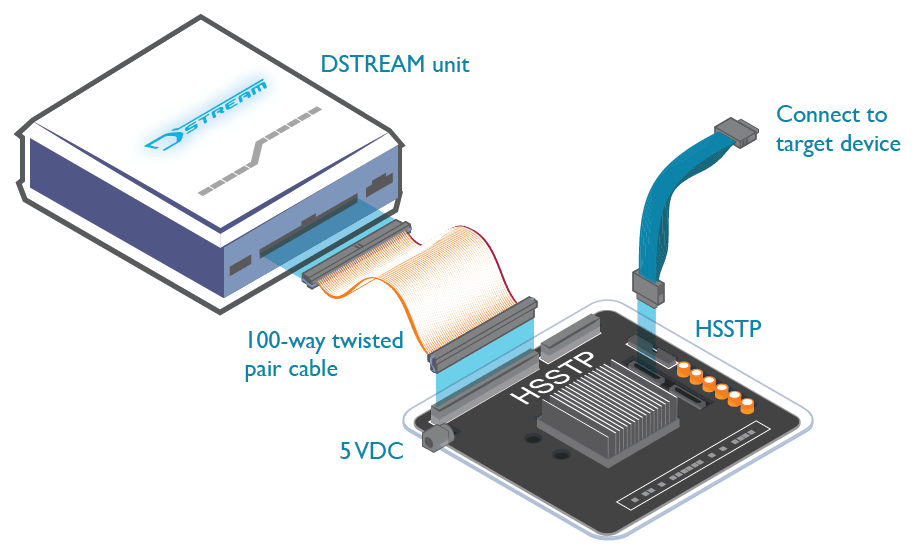
\includegraphics[width=5cm]{content/chapter_hardware_srv/dstream}
    }

    \column{6cm}
    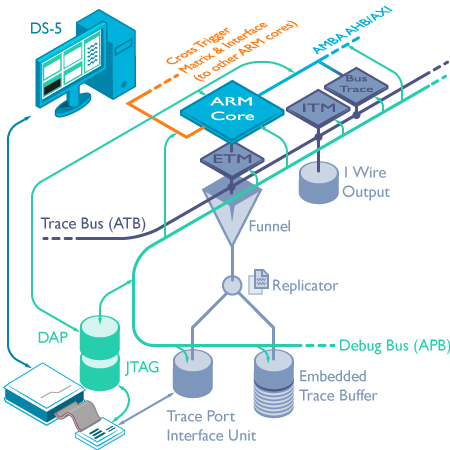
\includegraphics[width=6cm]{content/chapter_hardware_srv/coresight}
  \end{columns}
\end{frame}

\begin{frame}{Interactive Hardware Monitoring Workflow}
  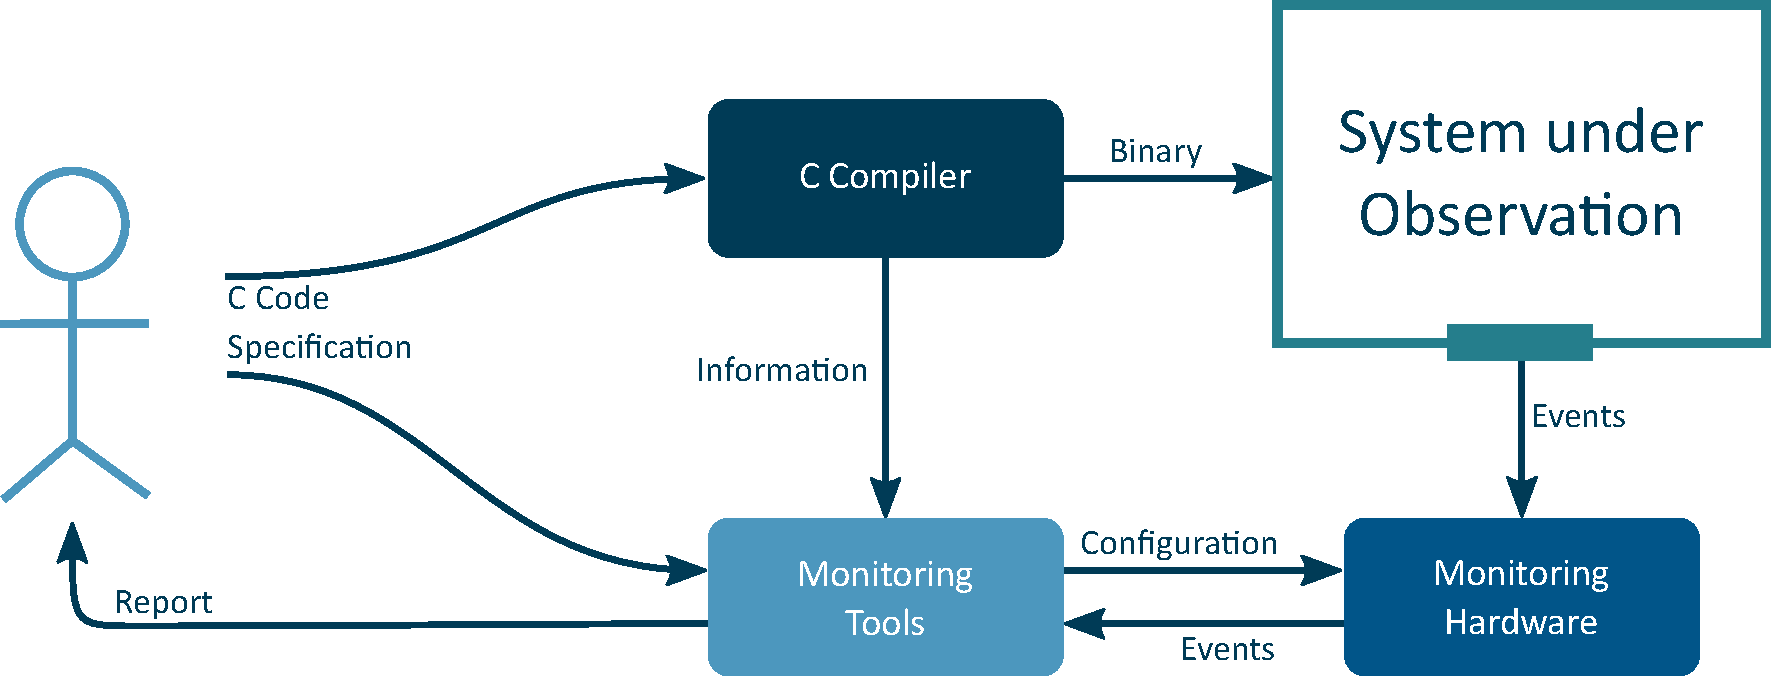
\includegraphics[width=\textwidth]{content/chapter_hardware_srv/overview-workflow.pdf}

  \vskip3ex\pause

  \alert{\large Fast reconfigurablility for interactive debugging sessions}

  \vskip3ex

  \begin{columns}
    \column{4.5cm}
    \inhead{Synthesized FPGA design}

    \begin{itemize}
      \item Trace Reconstruction\\\strut
      \item Monitoring Engine
    \end{itemize}

    \column{5cm}
    \inhead{configured through memory with}

    \begin{itemize}
      \item program binary\\
        (LUT of jumps)\strut
      \item monitoring specification
    \end{itemize}
  \end{columns}
\end{frame}

\begin{frame}
  \begin{center}
    \vskip-3ex
    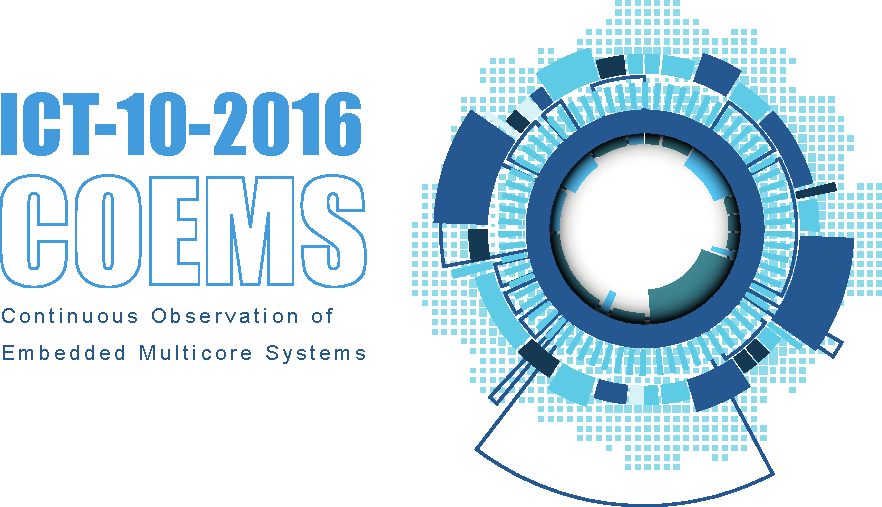
\includegraphics[width=7cm]{content/chapter_hardware_srv/logos/coems}

    \vskip1ex

    \raisebox{-0.5\height}{
\includegraphics[width=4cm]{content/chapter_hardware_srv/logos/isp-uni-luebeck}}
    \qquad
    \raisebox{-0.5\height}{
\includegraphics[width=4cm]{content/chapter_hardware_srv/logos/accemic}}

    \vskip1ex

    \raisebox{-0.5\height}{
\includegraphics[width=4cm]{content/chapter_hardware_srv/logos/airbus}}
    \qquad
    \raisebox{-0.5\height}{
\includegraphics[width=4cm]{content/chapter_hardware_srv/logos/hvl}}
    
    \vskip1ex

    
\includegraphics[width=4cm]{content/chapter_hardware_srv/logos/thales}
  \end{center}
\end{frame}

\begin{frame}{COEMS Hardware}
  \includegraphics[width=\textwidth]{content/chapter_hardware_srv/coems-hardware.pdf}
\end{frame}

\begin{frame}{COEMS Advantages}
  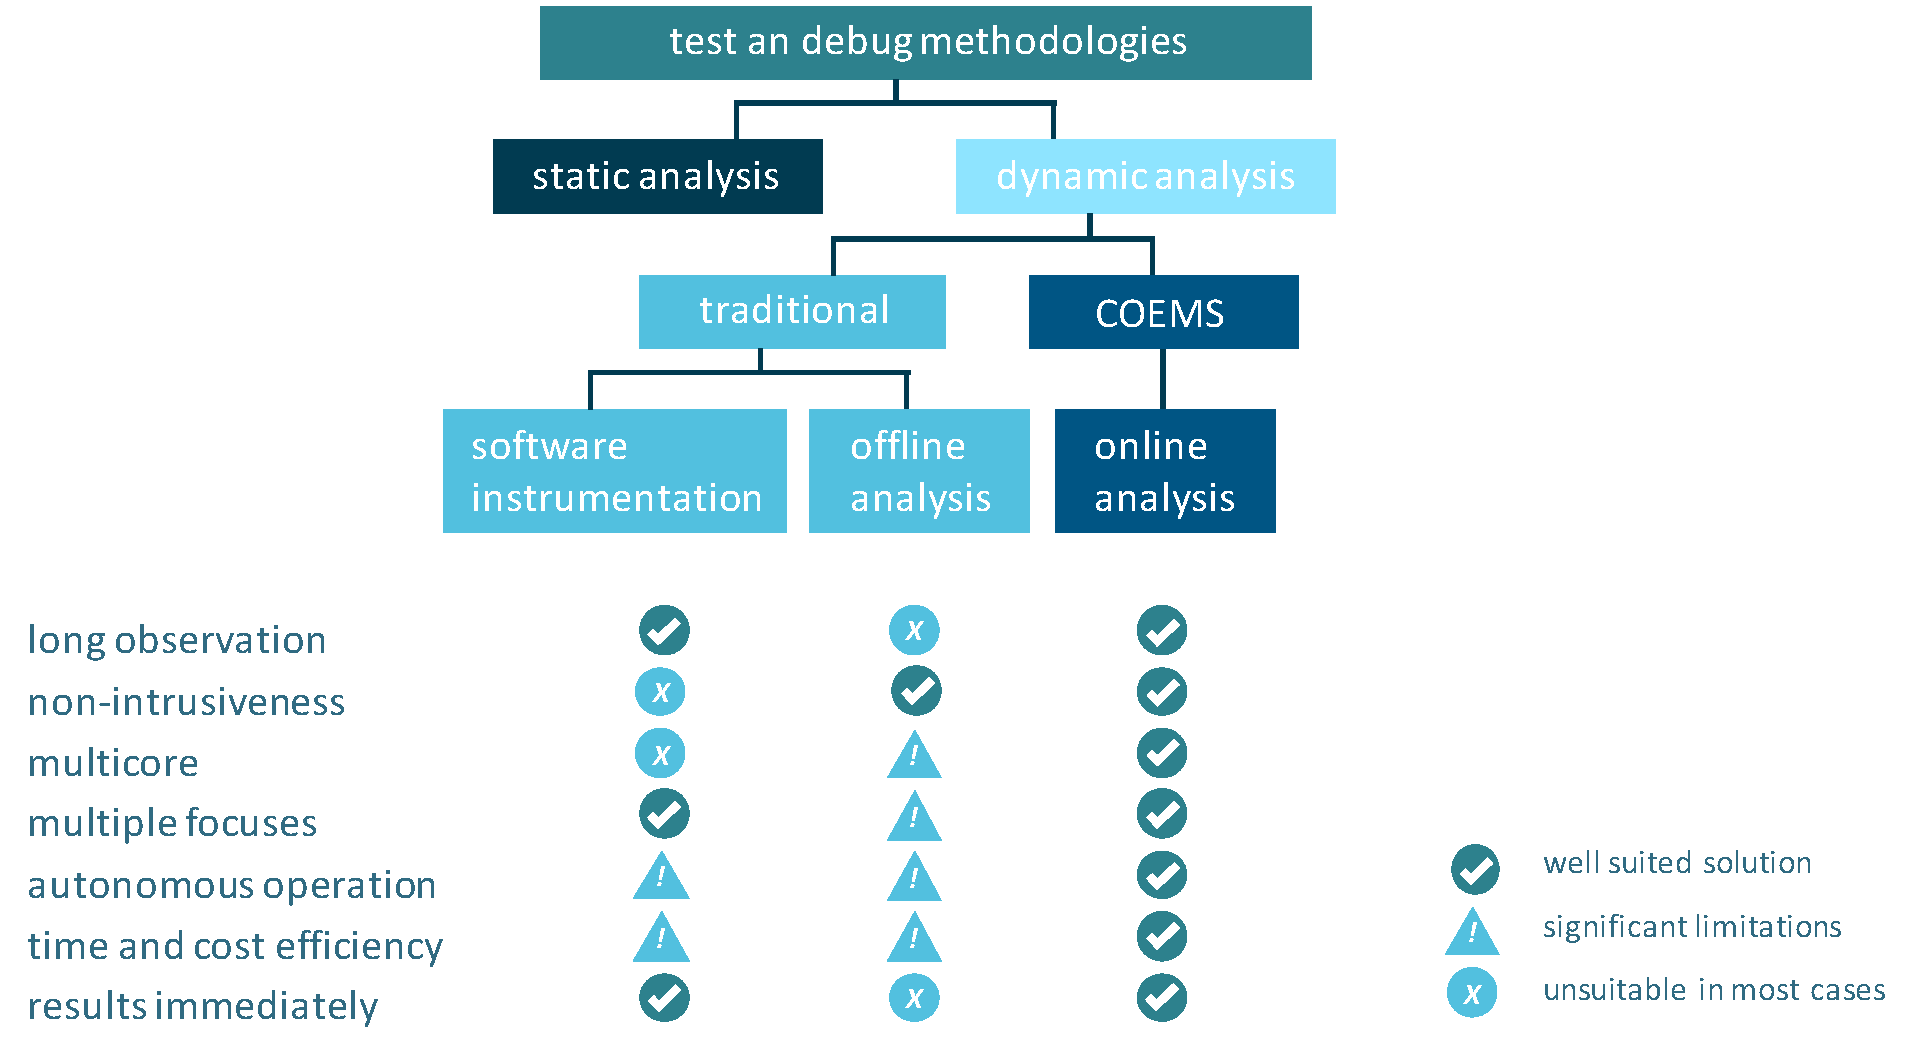
\includegraphics[width=\textwidth]{content/chapter_hardware_srv/coems-advantages.pdf}
\end{frame}